\chapter{Theoretical Background}
\label{cha:Theoretical}

This chapter provides an overview of the theoretical background relevant to steerable terrain generation using diffusion models. It covers the types of remote sensing data used for terrain modeling, key terrain features, the fundamentals of diffusion models, control methods for conditioning diffusion models, training objectives and optimization techniques, and evaluation metrics for assessing model performance.

\section{Remote Sensing Data for Terrain Modeling}
\label{subsec:remote_sensing_data}

Remote sensing data provides critical information about Earth's surface, enabling the analysis and modeling of terrain features. Satellite imagery offers high-resolution multispectral data that captures both surface appearance and structural characteristics.

\subsection{Sentinel-2 Optical Imagery}
\label{subsec:sentinel2_optical_imagery}

Sentinel-2 is a key satellite mission operated by the European Space Agency that delivers high-resolution multispectral optical imagery across 13 spectral bands in the visible to shortwave infrared range. With spatial resolutions up to 10 meters and a revisit period of 5 days, Sentinel-2 has become a core source of surface reflectance data for land cover monitoring. Its bands are distributed across three resolution tiers: 4 bands at 10 m (blue, green, red, NIR), 6 bands at 20 m, and 3 bands at 60 m, making it highly flexible as a source of surface appearance for terrain generation tasks. It is organized into a fixed tiling grid, where each tile covers a 100 by 100 km area~\cite{drusch2012sentinel2, falkner2025sentinel2tiling}.

\subsection{Digital Elevation Models}
\label{subsec:digital_elevation_models}

DEMs are raster-based representations of terrain elevation, structured as a continuous grid of elevation values. DEMs are derived from various sources, including satellite radar, LiDAR, and photogrammetry. They provide critical information about terrain structure, enabling the extraction of geomorphological features such as slope, aspect, curvature, ridges, valleys, and cliffs~\cite{pike2008guide}.

\section{Features of Terrain}
\label{sec:terrain_features}

There are several key features of terrain that are commonly extracted from DEMs and used in terrain analysis and modeling. These include slope which measures the steepness of the terrain, ridges which are linear high points that divide drainage basins, valleys which are linear low points that concentrate water flow, cliffs or escarpments which are regions of abrupt elevation change, and flats or plateaus which are low-curvature areas at elevated positions~\cite{pike2008guide, hengl2008geomorphometry}.

\section{Diffusion Models}
\label{subsec:diffusion_models}

Diffusion models generate data by reversing a gradual noising process learning to denoise samples step by step. Introduced by Sohl-Dickstein et al.~\cite{sohl2015deep} and popularized by Ho et al.~\cite{ho2020ddpm}, diffusion models have emerged as powerful generative models capable of producing high-quality images and other data modalities.

\subsection{Diffusion Process}
\label{subsec:diffusion_process}

\subsubsection{Forward Diffusion Process}
\label{subsubsec:forward_diffusion_process}

In the forward process, a clean data sample $\mathbf{x}_0$ is progressively corrupted by the addition of Gaussian noise over $T$ discrete time steps. At each step $t$, a small amount of noise is added, resulting in a sequence $\mathbf{x}_0, \mathbf{x}_1, \ldots, \mathbf{x}_T$, where $\mathbf{x}_T$ approaches pure noise. This process is modeled as a Markov chain:
\[
	q(\mathbf{x}_t | \mathbf{x}_{t-1}) = \mathcal{N}(\mathbf{x}_t;\mathbf{x}_{t-1} \sqrt{1 - \beta_t}, \mathbf{I} \beta_t)
\]
where $\beta_t$ is a variance schedule controlling the noise level at each step.

The entire forward process can be expressed in closed form as:
\[
	q(\mathbf{x}_t | \mathbf{x}_0) = \mathcal{N}(\mathbf{x}_t; \sqrt{\bar{\alpha}_t}\,\mathbf{x}_0, (1 - \bar{\alpha}_t)\mathbf{I})
\]
with $\bar{\alpha}_t = \prod_{s=1}^t (1 - \beta_s)$~\cite{ho2020ddpm}.

\subsubsection{Reverse Diffusion Process}
\label{subsubsec:reverse_diffusion_process}

Diffusion models work by learning the reverse process. The model denoises a sample starting from pure noise $\mathbf{x}_T$ to recover a realistic data point.
This reverse process is also modeled as a Markov chain:
\[
	p_\theta(\mathbf{x}_{t-1} | \mathbf{x}_t) = \mathcal{N}(\mathbf{x}_{t-1}; \boldsymbol{\mu}_\theta(\mathbf{x}_t, t), \Sigma_\theta(\mathbf{x}_t, t))
\]
where $\boldsymbol{\mu}_\theta$ and $\Sigma_\theta$ are predicted by the network, conditioned on the current noisy sample and the timestep $t$~\cite{ho2020ddpm}.

\subsubsection{Training Objective}
\label{subsubsec:training_objective}

Diffusion models are trained to predict either the added noise or the original clean sample at each step. The most common loss introduced by Ho et al.~\cite{ho2020ddpm} is the mean squared error between the true noise $\boldsymbol{\epsilon}$ and the model's prediction $\boldsymbol{\epsilon}_\theta$:
\[
	L_{\text{simple}} = \mathbb{E}_{\mathbf{x}_0, \boldsymbol{\epsilon}, t} \left[ \left\| \boldsymbol{\epsilon} - \boldsymbol{\epsilon}_\theta(\mathbf{x}_t, t) \right\|^2 \right]
\]
where $\mathbf{x}_t = \sqrt{\bar{\alpha}_t}\,\mathbf{x}_0 + \sqrt{1 - \bar{\alpha}_t}\,\boldsymbol{\epsilon}$.

\subsubsection{Improvements and Variants}
\label{subsubsec:improvements_variants}

Subsequent work has introduced improvements to the basic diffusion process such as learning the variance schedule~\cite{nichol2021improved}, improved sampling procedures~\cite{song2021denoising} and architectural enhancements that enable diffusion models to surpass GANs in image synthesis quality~\cite{dhariwal2021diffusion}.

\subsubsection{U-Net Architecture}
\label{subsubsec:unet_architecture}

U-Net is a convolutional neural network architecture widely used as the backbone for diffusion models due to its ability to capture multi-scale features through an encoder-decoder structure with skip connections. Originally proposed by Ronneberger et al.~\cite{ronneberger2015unet} for biomedical image segmentation, U-Net has been adapted for diffusion models by Ho et al.~\cite{ho2020ddpm}. The U-Net architecture consists of an encoder and a decoder. The encoder progressively reduces the spatial dimensions of the input while increasing the number of feature channels capturing high-level semantic information. The decoder then upsamples the feature maps back to the original resolution to reconstruct the output. Skip connections between corresponding layers in the encoder and decoder allow the model to retain information. In diffusion models, the U-Net takes the noisy sample $\mathbf{x}_t$ and the timestep $t$ as input. The network predicts either the noise component or the denoised sample at each step of the reverse diffusion process.

\begin{figure}[htbp]
	\centering
	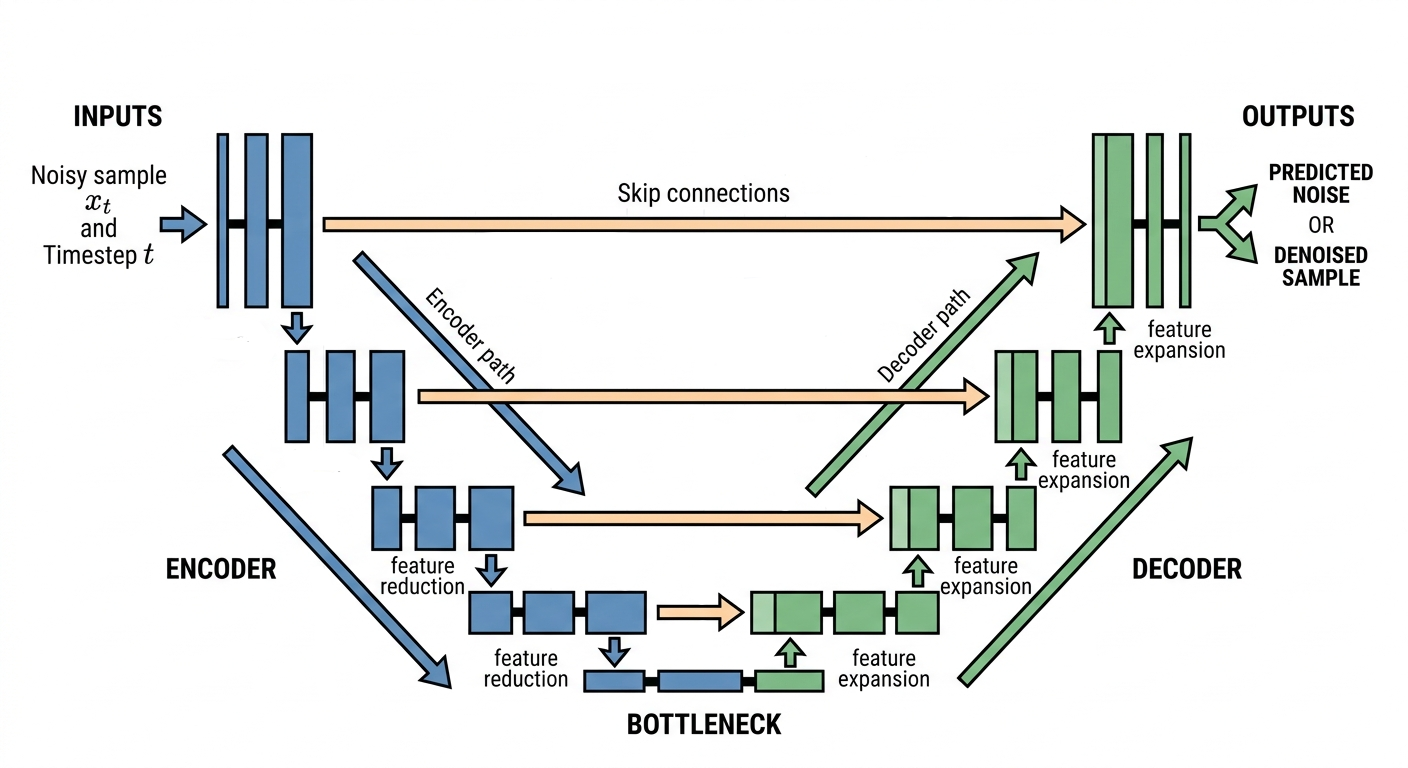
\includegraphics[width=\linewidth]{images/unet.png}
	\caption{Diagram of the U-Net architecture used in diffusion models, showing the encoder, decoder, and skip connections.}
	\label{fig:unet}
\end{figure}

\subsubsection{Latent Diffusion}
\label{subsubsec:latent_diffusion}

Latent Diffusion Models are a variant of diffusion models that first compress the image into a lower-dimensional latent space before performing the diffusion process. Introduced by Rombach et al.~\cite{rombach2022stable}, Latent Diffusion Models leverage a pretrained autoencoder, typically a Variational Autoencoder~\cite{kingma2014auto}, to encode the images into a latent representation. The autoencoder consists of an encoder that maps the input image to a latent vector and a decoder that reconstructs the image from the latent vector. The diffusion model is trained to denoise latent vectors instead of images allowing for faster training and inference.

\begin{figure}[htbp]
	\centering
	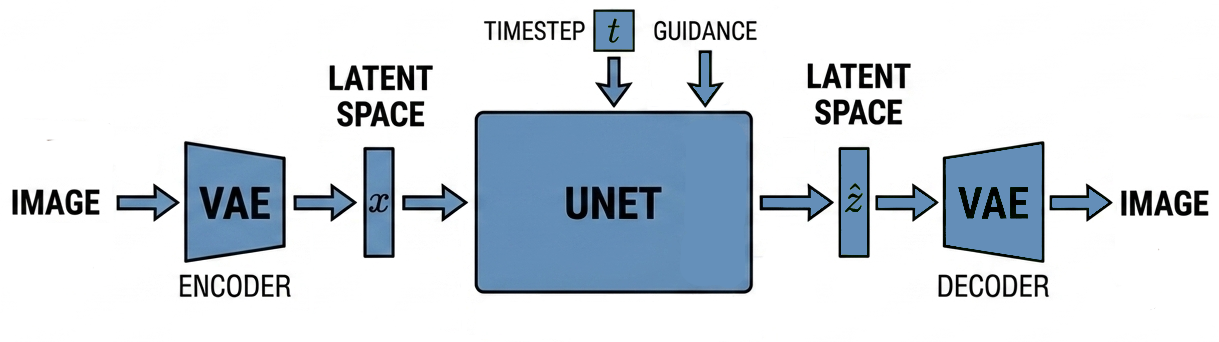
\includegraphics[width=\linewidth]{images/latent_unet.png}
	\caption{Diagram illustrating the architecture of a Latent Diffusion Model, showing the autoencoder and the diffusion process in the latent space.}
	\label{fig:latent_unet}
\end{figure}

\section{Control Methods for Diffusion Models}
\label{sec:control_methods}

Controlling diffusion models is crucial for applications requiring precise feature placement, such as terrain generation. Although existing diffusion models already support conditioning methods via cross attention layers these need to be incorporated during the initial training of the diffusion model. To enable conditioning on additional modalities without having to retrain the entire model, which is computationally expensive, ControlNet~\cite{zhang2023controlnet} and T2I-Adapter~\cite{mou2023t2i} have been proposed. Both methods allow for conditioning on various input modalities while preserving the capabilities of pretrained diffusion models.

\subsection{ControlNet}
\label{subsec:controlnet}

ControlNet adds additional control modalities to pretrained diffusion models by creating a trainable copy of the model's encoder layers. This copy is connected to the original network via zero-initialized convolutional layers allowing it to learn condition-specific features while preserving the weights of the pretrained model. During training, the original diffusion model remains frozen and only the ControlNet layers are updated. This approach enables strong conditioning control while preserving the capabilities of the original model albeit with computational overhead due to the network duplication~\cite{zhang2023controlnet}.

\begin{figure}[htbp]
	\centering
	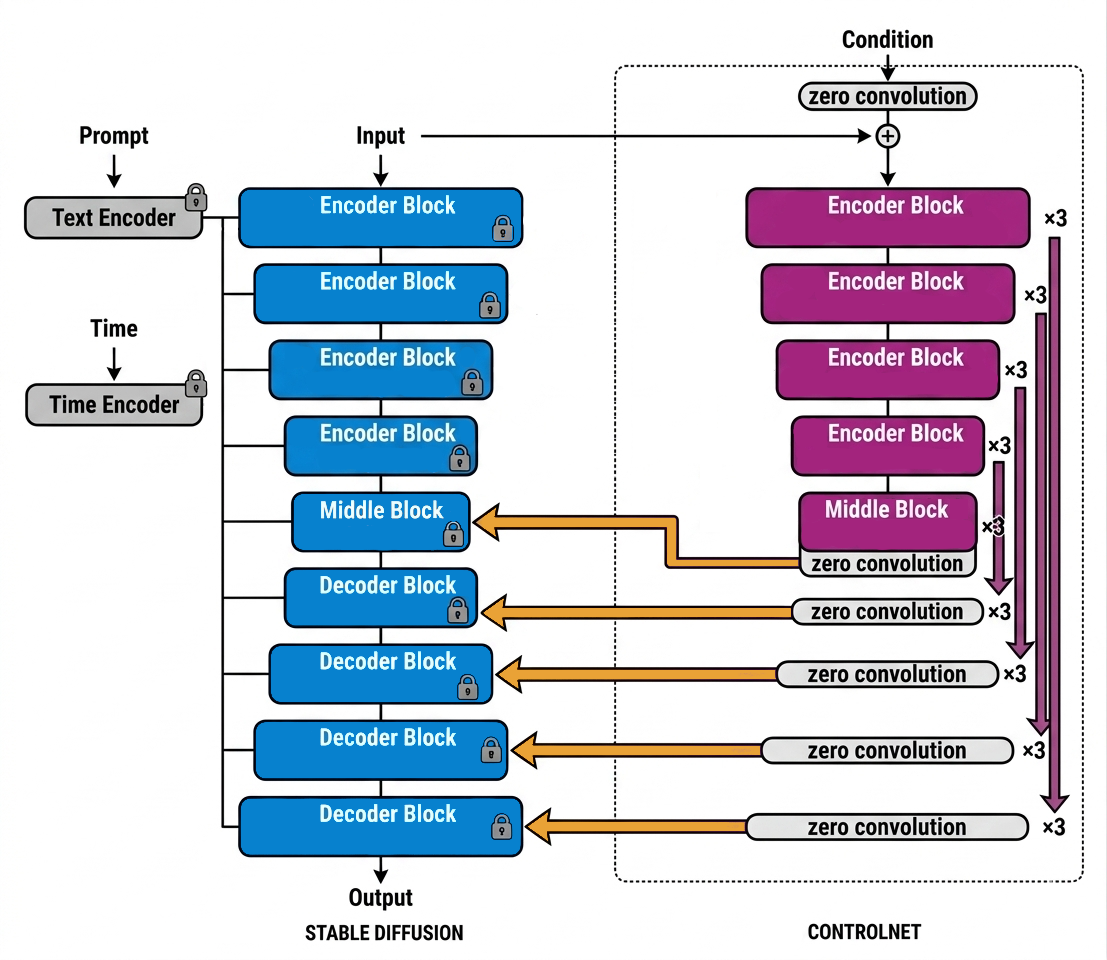
\includegraphics[width=\linewidth]{images/controlnet.png}
	\caption{Diagram illustrating the ControlNet architecture, showing the original diffusion model and the additional control layers.}
	\label{fig:controlnet}
\end{figure}

\subsection{T2I Adapter}
\label{subsec:t2i_adapter}

T2I-Adapter proposes a lightweight alternative to ControlNet by introducing small adapters that can be integrated into pretrained diffusion models. Instead of duplicating the entire network, T2I-Adapter uses adapters that extract features from the control conditions and progressively integrate them into the diffusion process This design significantly reduces the number of additional parameters and computational requirements compared to ControlNet while still providing effective conditioning capabilities~\cite{mou2023t2i}.

\begin{figure}[htbp]
	\centering
	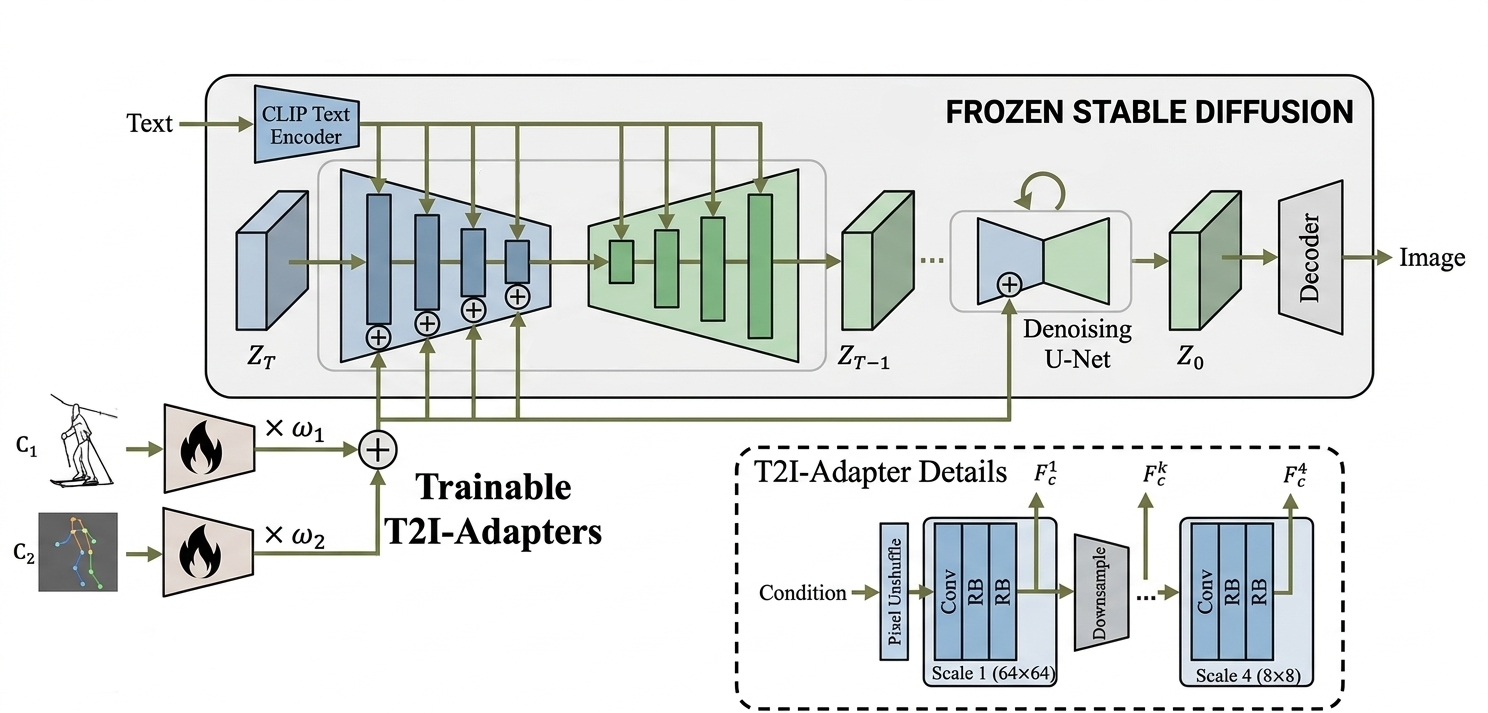
\includegraphics[width=\linewidth]{images/t2i.png}
	\caption{Diagram illustrating the T2I-Adapter architecture, showing the original diffusion model and the adapter layers.}
	\label{fig:t2i_adapter}
\end{figure}

\subsection{Comparison of Control Architectures}
\label{subsec:comp_control}

ControlNet and T2I-Adapter represent two distinct approaches to adding spatial control to pretrained diffusion models. ControlNet involves duplicating the entire encoder network resulting in significant computational overhead during training. In contrast, T2I-Adapter employs an lightweight adapter that introduces far fewer parameters making it more efficient in terms of training time and resource usage. Both methods have demonstrated strong conditioning capabilities, but they differ in terms of control fidelity, generation quality and integration complexity.

\section{Training Objectives and Optimization}
\label{subsec:training_objectives_optimization}

\subsection{AdamW Optimizer}
\label{subsec:adam_optimizer}

AdamW is an optimization algorithm that combines the benefits of the Adam optimizer with decoupled weight decay regularization. Introduced by Loshchilov et al.~\cite{loshchilov2019adamw}, AdamW addresses the issue of L2 regularization being coupled with the adaptive learning rates in Adam, which can lead to suboptimal convergence. By decoupling weight decay from the gradient updates, AdamW allows for more effective regularization and improved generalization performance in training deep neural networks.

\subsection{Prodigy Optimizer}
\label{subsec:prodigy_optimizer}

Prodigy is an optimization algorithm designed for training large-scale deep learning models. Introduced by Mishchenko and Defazio~\cite{mishchenko2023prodigy}, Prodigy combines the advantages of adaptive gradient methods with momentum-based optimization to achieve faster convergence and improved performance. Prodigy incorporates a dynamic learning rate schedule and adaptive momentum to effectively navigate the loss landscape, making it particularly well-suited for training complex models such as diffusion models without having to tune or sweep the learning rate.

\section{SNR Weighted Loss}
\label{sec:snr_weighted_loss}

SNR Weighted Loss is a training objective for diffusion models that weights the loss based on the signal-to-noise ratio (SNR) of the noisy samples at each timestep. Introduced by Hang et al.~\cite{hang2024efficientdiffusiontrainingminsnr}, this approach addresses the issue of imbalanced training across different noise levels by giving more emphasis to samples with higher SNR, which are typically more informative for learning.

\section{Evaluation Metrics}
\label{subsec:evaluation_metrics}

\subsection{Mean Intersection over Union}
\label{subsec:miou}

Mean Intersection over Union (mIoU) is a common evaluation metric used in image segmentation tasks to measure the overlap between predicted segmentation masks and ground truth masks. It is calculated as the average of the Intersection over Union (IoU) across all classes, where IoU is defined as the ratio of the area of overlap between the predicted and ground truth masks to the area of their union. mIoU provides a comprehensive measure of segmentation accuracy, accounting for both false positives and false negatives, making it a standard metric for evaluating segmentation performance~\cite{long2015fully}.
